\def\pgfsysdriver{pgfsys-dvisvgm.def}
% flashcards-title: Evidence convergence, conflict, and claim revision
% flashcards-desc: Two separate evidence boxes point to a bounded claim. A conflicting result points to checking conditions, which points to a revised bounded claim.
\documentclass[tikz,border=6pt]{standalone}
\usetikzlibrary{arrows.meta,calc,fit,positioning,shapes.geometric}

\definecolor{fcink}{HTML}{17212B}
\definecolor{fcblue}{HTML}{1D5D8C}
\definecolor{fcgreen}{HTML}{2D6A4F}
\definecolor{fcorange}{HTML}{A44A1F}
\definecolor{fcpale}{HTML}{F4F7F9}
\definecolor{fcsoil}{HTML}{8B5E3C}

\tikzset{
  fc text/.style={font=\sffamily, text=fcink},
  fc panel/.style={draw=fcink, line width=0.9pt, rounded corners=5pt, fill=fcpale},
  fc node/.style={draw=fcink, line width=0.9pt, rounded corners=4pt, fill=white,
    minimum width=24mm, minimum height=10mm, align=center, font=\sffamily},
  fc arrow/.style={-{Stealth[length=3.2mm,width=2.4mm]}, line width=1.2pt,
    draw=fcblue, line cap=butt},
  fc boundary/.style={draw=fcorange, line width=1.4pt, dash pattern=on 5pt off 3pt,
    rounded corners=7pt},
  fc label/.style={font=\sffamily\bfseries, text=fcink},
  fc note/.style={font=\sffamily\small, text=fcink, align=center}
}

\begin{document}
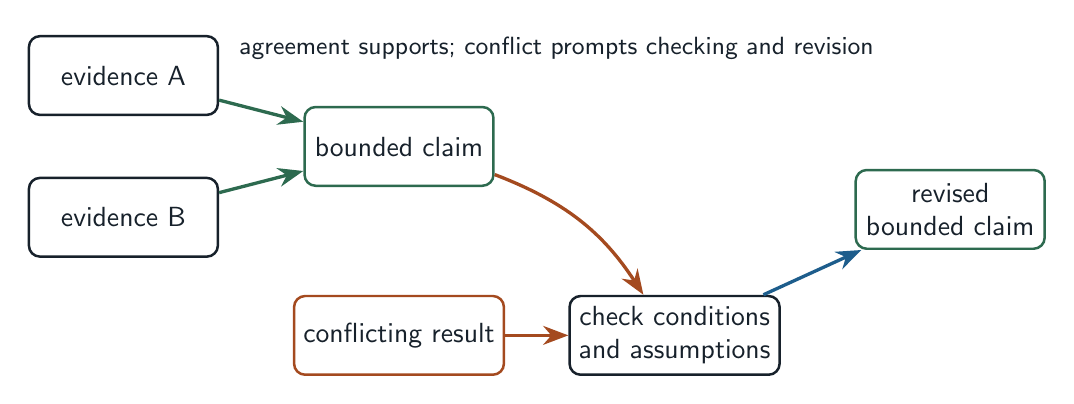
\begin{tikzpicture}[fc text, x=1cm, y=1cm]
  \node[fc node] (e1) at (1.7,4.1) {evidence A};
  \node[fc node] (e2) at (1.7,2.3) {evidence B};
  \node[fc node, draw=fcgreen] (claim) at (5.2,3.2) {bounded claim};
  \draw[fc arrow, draw=fcgreen] (e1)--(claim);
  \draw[fc arrow, draw=fcgreen] (e2)--(claim);
  \node[fc node, draw=fcorange] (conf) at (5.2,.8) {conflicting result};
  \node[fc node] (check) at (8.7,.8) {check conditions\\and assumptions};
  \node[fc node, draw=fcgreen] (rev) at (12.2,2.4) {revised\\bounded claim};
  \draw[fc arrow, draw=fcorange] (conf)--(check);
  \draw[fc arrow] (check)--(rev);
  \draw[fc arrow, draw=fcorange, bend left=18] (claim) to (check);
  \node[fc note] at (7.2,4.45) {agreement supports; conflict prompts checking and revision};
\end{tikzpicture}
\end{document}
